
\begin{lead}

 信号をフーリエ解析する際に,\index{DFT@DFT}DFTは必ず知っておく必要があるとされている.ところが,実際にコンピュータ上での演算や,\index{はーどうぇあじっそう@ハードウェア実装}ハードウェア実装を行うにあたっては,\index{けいさんじかん@計算時間}計算時間や\index{けいさんこすと@計算コスト}計算コストが非常に大きいという問題があった.
%
もし同じ計算結果を得ることができるのであれば,可能な限り,計算時間や計算コストが少なくなるようなアルゴリズムによる計算方法が望ましい.

 このことから,フーリエ変換の計算を行う際に計算コストをできる限り少なくするための\index{こうそくふーりえへんかん@高速フーリエ変換}高速フーリエ変換 (Fase Fourier Transform: FFT) のアルゴリズムが研究された.

 本章では,実用上重要な\index{FFT@FFT}FFTのアルゴリズムを解説する.

\end{lead}

%\vfill

%\begin{koumoku}
%高速フーリエ変換(FFT)\\
%複素指数関数\\
%位相回転因子\\
%時間間引き\\
%乗算回数
%\end{koumoku}

%\clearpage

\chapter{高速フーリエ変換}
\label{chapter:fft}

\section{高速フーリエ変換の原理}

DFTによるフーリエ係数の計算式は,
\begin{equation}
C_k=\frac{1}{N}\sum^{N-1}_{i=0}x[i] e^{-j\frac{2\pi}{N}ki}
\label{eqn:dft51}
\end{equation}
である.ここで,以下に示すような\index{ふくそしすうかんすう@複素指数関数}複素指数関数$W$について見てみることにする.
\begin{equation}
W=e^{-j\frac{2\pi}{N}} = \cos \frac{2\pi}{N} -j\sin \frac{2\pi}{N}
\end{equation}
 ところで,$n=ki$とすると,$W^i$は図\ref{fig:isou_kaiten}に示すように複素平面の原点中心に単位円の円周上を$N$等分した点を表し,その点は$n$の増加とともに負方向(時計回り)に$1/N$刻みで回転する.このことから,$W$は位相回転因子と呼ばれる.図\ref{fig:isou_kaiten}のように$N=8$の場合,
\begin{equation}
W^8=W^0, W^9=W^1, \cdots \nonumber
\end{equation}
なる周期性が存在する.この周期性を一般式で示すと,次式のようになる.
\begin{equation}
W^n=W^{n\rm{mod}N}
\end{equation}
ここで,$n\rm{mod}N$は$n$を$N$で割った余りを意味する.

\begin{figure}[H]
\begin{center}
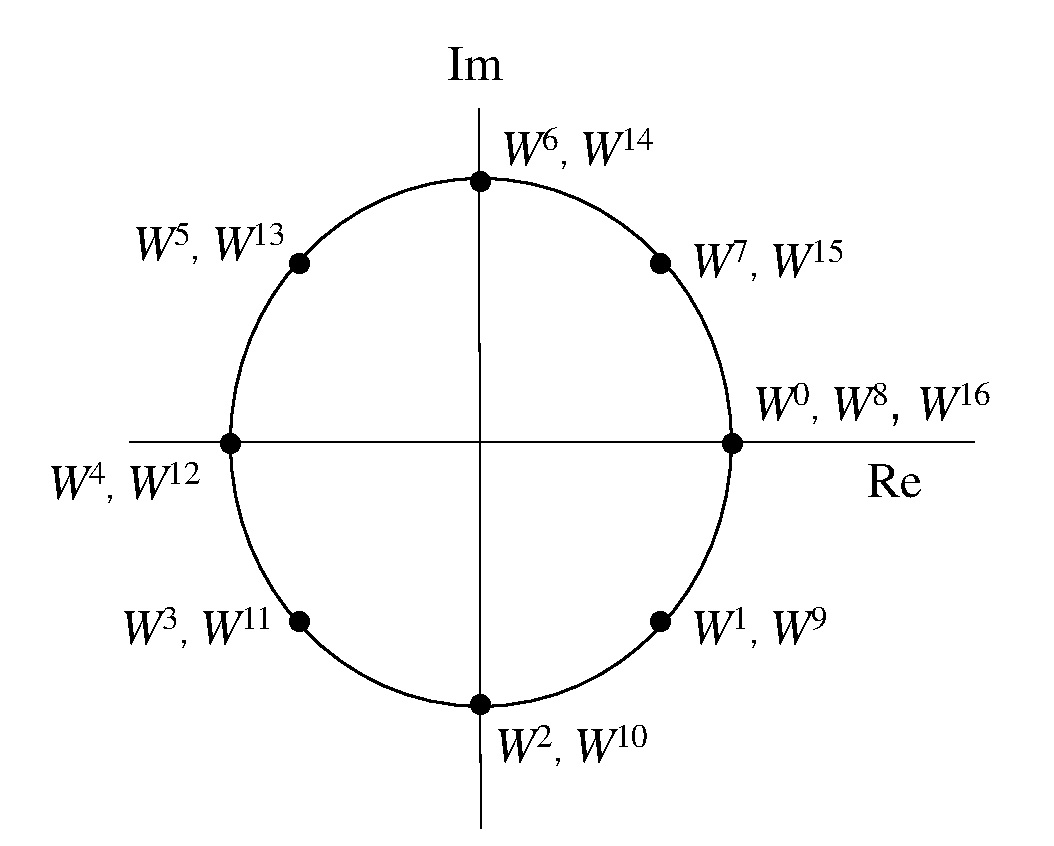
\includegraphics[width=.6\textwidth]{fig/isou_kaiten.eps}
\end{center}
\caption{位相回転因子$W$のべき乗($N=8$)}
\label{fig:isou_kaiten}
\end{figure}

また,$W^4=-W^0$,$W^5=-W^1 \cdots$のような\index{たいしょうせい@対称性}対称性も存在することから,
\begin{equation}
W^n=-W^{ n -N/2 }
\end{equation}
と示すことができる.このように$W^n$の\index{しゅうきせい@周期性}周期性と対称性を利用することで,DFTに必要な乗算回数を大幅に減少できると考えられる.

さて,\index{いそうかいてんいんし@位相回転因子}位相回転因子$W$を用いてDFTの式(式(\ref{eqn:dft51}))を書き換えると,
\begin{equation}
\begin{bmatrix}
C_0 \\
C_1 \\
C_2 \\
C_3
\end{bmatrix}
=
\begin{bmatrix}
W^0 & W^0 & W^0 & W^0 \\
W^0 & W^1 & W^2 & W^3 \\
W^0 & W^2 & W^4 & W^6 \\
W^0 & W^3 & W^6 & W^9
\end{bmatrix}
\begin{bmatrix}
x[0] \\
x[1] \\
x[2] \\
x[3]
\end{bmatrix}
\label{eqn:dft55}
\end{equation}
となる.ここで,偶数番目のグループ$\{x[0], x[2] \}$と奇数番目のグループ$\{x[1], x[3] \}$に行列を分割すると,次式のように書き表すことができる.

\begin{eqnarray}
\begin{bmatrix}
C_0 \\
C_1 \\
C_2 \\
C_3
\end{bmatrix}
&=&
\begin{bmatrix}
W^0 & W^0 & W^0 & W^0 \\
W^0 & W^2 & W^1 & W^3 \\
W^0 & W^4 & W^2 & W^6 \\
W^0 & W^6 & W^3 & W^9
\end{bmatrix}
\begin{bmatrix}
x[0] \\
x[2] \\
x[1] \\
x[3]
\end{bmatrix}
\\
&=&
\begin{bmatrix}
W^0 & W^0 \\
W^0 & W^2 \\
W^0 & W^4 \\
W^0 & W^6
\end{bmatrix}
\begin{bmatrix}
x[0] \\
x[2]
\end{bmatrix}
+
\begin{bmatrix}
W^0 & W^0 \\
W^1 & W^3 \\
W^2 & W^6 \\
W^3 & W^9
\end{bmatrix}
\begin{bmatrix}
x[1] \\
x[3]
\end{bmatrix}
\\
&=&
\begin{bmatrix}
W^0 & W^0 \\
W^0 & W^2 \\
W^0 & W^4 \\
W^0 & W^6
\end{bmatrix}
\begin{bmatrix}
x[0] \\
x[2]
\end{bmatrix}
+
\begin{bmatrix}
W^0 \\
W^1 \\
W^2 \\
W^3 
\end{bmatrix}
\begin{bmatrix}
W^0 & W^0 \\
W^0 & W^2 \\
W^0 & W^4 \\
W^0 & W^6
\end{bmatrix}
\begin{bmatrix}
x[1] \\
x[3]
\end{bmatrix}
\\
&=&
\begin{bmatrix}
1 & W^0 \\
1 & -W^0 \\
1 & W^0 \\
1 & -W^0
\end{bmatrix}
\begin{bmatrix}
x[0] \\
x[2]
\end{bmatrix}
+
\begin{bmatrix}
W^0 \\
W^1 \\
W^2 \\
W^3 
\end{bmatrix}
\begin{bmatrix}
1 & W^0 \\
1 & -W^0 \\
1 & W^0 \\
1 & -W^0
\end{bmatrix}
\begin{bmatrix}
x[1] \\
x[3]
\end{bmatrix}
\label{eqn:dft56}
\end{eqnarray}\vskip.3\baselineskip

式(\ref{eqn:dft56})については,図\ref{fig:バタフライ}に示すような\index{ばたふらいえんざん@バタフライ演算}バタフライ演算を用いて計算過程を考える.
すると,式(\ref{eqn:dft56})における\index{まとりくす@マトリクス}マトリクスとデータとの乗算部分については図\ref{fig:バタフライ1}のように示すことができる.

\begin{figure}[H]
\begin{center}
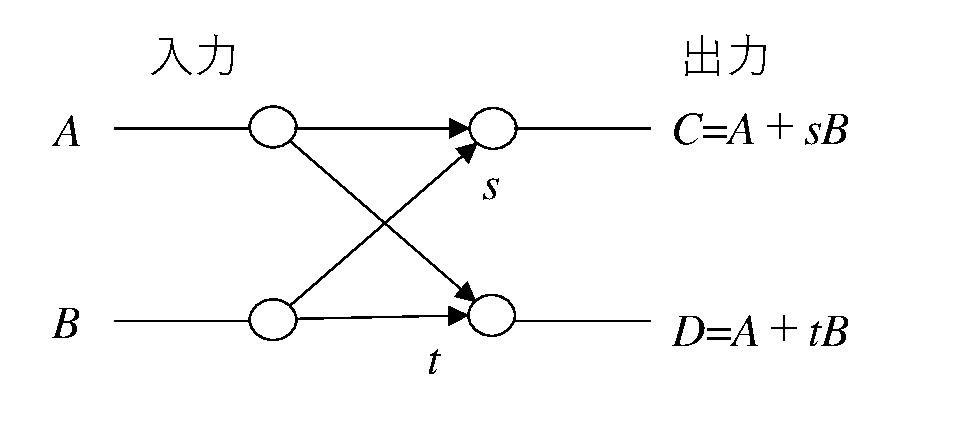
\includegraphics[width=.6\textwidth]{fig/butterfly1.eps}
\end{center}
\caption{バタフライ演算の規則}
\label{fig:バタフライ}
\end{figure}


\begin{figure}[H]
\begin{center}
\includegraphics[width=.6\textwidth]{fig/butterfly2.eps}

(a) 式(\ref{eqn:dft56})右辺の第1項の部分の上段と下段
\end{center}\vskip.5\baselineskip

\begin{center}
\includegraphics[width=.6\textwidth]{fig/butterfly3.eps}

(b) 式(\ref{eqn:dft56})の右辺の第2項の部分の上段と下段
\end{center}\vskip.5\baselineskip
\caption{初回のバタフライ演算}
\label{fig:バタフライ1}
\end{figure}

このように,1つのバタフライ演算では符号が異なるだけで1つの入力データに同じ係数が掛けられていることから,1回のバタフライ演算では1回の乗算で済むことがわかる.すなわち,1回目のバタフライ演算の出力結果を,$\{ C_1', C_2', C_3', C_4'\}$とすれば,式(\ref{eqn:dft56})は次式のように書くことができる.

\begin{eqnarray}
\begin{bmatrix}
C_0 \\
C_1 \\
C_2 \\
C_3
\end{bmatrix}
&=&
\begin{bmatrix}
C_0' \\
C_1' \\
C_0' \\
C_1'
\end{bmatrix}
+
\begin{bmatrix}
W^0 \\
W^1 \\
-W^0 \\
-W^1
\end{bmatrix}
\begin{bmatrix}
C_2' \\
C_3' \\
C_2' \\
C_3'
\end{bmatrix}
\label{eqn:dft57}
\end{eqnarray}\vskip.3\baselineskip

また,この式を2つのグループに分割すると,次式のようになる.

\begin{eqnarray}
\begin{bmatrix}
C_0 \\
C_2
\end{bmatrix}
&=&
\begin{bmatrix}
C_0' \\
C_0' \\
\end{bmatrix}
+
\begin{bmatrix}
W^0 \\
-W^0 \\
\end{bmatrix}
\begin{bmatrix}
C_2' \\
C_3'
\end{bmatrix}
\\
&=&
\begin{bmatrix}
1 & W^0 \\
1 & -W^0
\end{bmatrix}
\begin{bmatrix}
C_2' \\
C_3'
\end{bmatrix}
\label{eqn:dft58}
\end{eqnarray}\vskip.3\baselineskip

\begin{eqnarray}
\begin{bmatrix}
C_1 \\
C_3
\end{bmatrix}
&=&
\begin{bmatrix}
C_1' \\
C_1'
\end{bmatrix}
+
\begin{bmatrix}
W^1 \\
-W^1
\end{bmatrix}
\begin{bmatrix}
C_3' \\
C_3'
\end{bmatrix}
\\
&=&
\begin{bmatrix}
1 & W^1 \\
1 & -W^1
\end{bmatrix}
\begin{bmatrix}
C_1' \\
C_3'
\end{bmatrix}
\label{eqn:dft581}
\end{eqnarray}\vskip.3\baselineskip

この式(\ref{eqn:dft58}),式(\ref{eqn:dft581})をまとめて図示すると,図\ref{fig:バタフライ2}のようになる.
さらに,図\ref{fig:バタフライ1}と図\ref{fig:バタフライ2}をまとめると図\ref{fig:バタフライ3}のように書き表すことができる.このように2回のバタフライ演算のペアは,2段ずれたデータと組まれていることに注意すれば,FFTの概念は図\ref{fig:バタフライ3}のようにまずデータを並び換えて,次にバタフライ演算を次々に実行する,というように行われることがわかる.

\begin{figure}[H]
\begin{center}
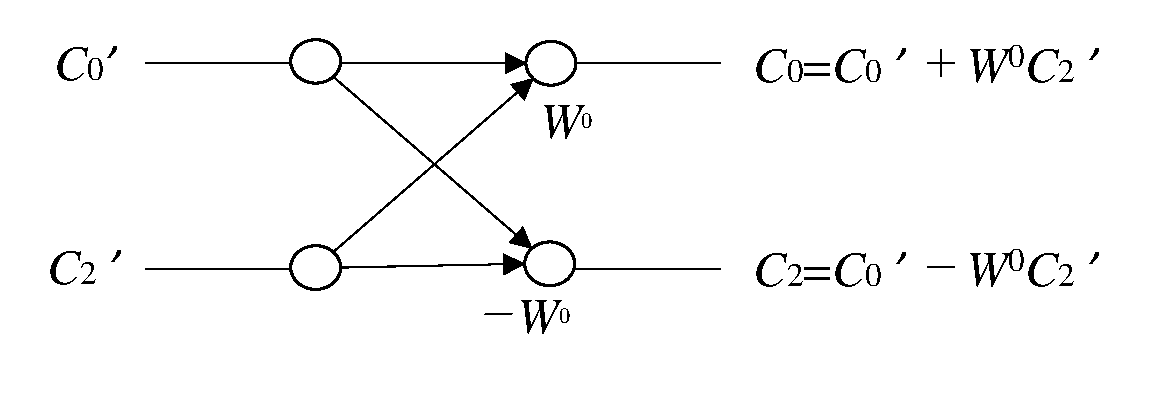
\includegraphics[width=.6\textwidth]{fig/butterfly4.eps}

(a) 式(\ref{eqn:dft58})の右辺の上段と下段
\end{center}\vskip.5\baselineskip

\begin{center}
\includegraphics[width=.6\textwidth]{fig/butterfly5.eps}

(b) 式(\ref{eqn:dft581})の右辺の上段と下段
\end{center}\vskip.5\baselineskip

\caption{式(\ref{eqn:dft57})のバタフライ演算}
\label{fig:バタフライ2}
\end{figure}



\begin{figure}[H]
\begin{center}
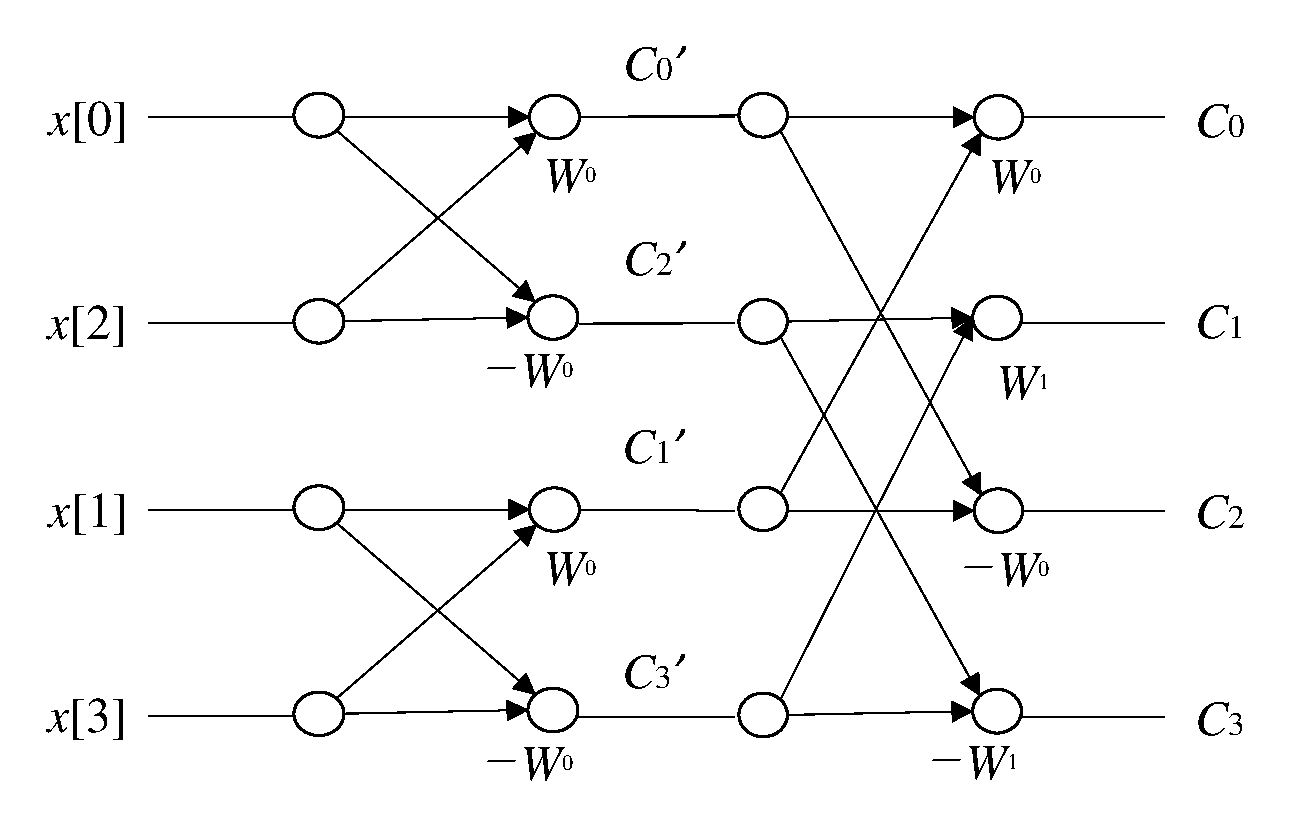
\includegraphics[width=.6\textwidth]{fig/butterfly6.eps}
\end{center}
\caption{4点FFTにおける全体のバタフライ演算}
\label{fig:バタフライ3}
\end{figure}

\section{FFTのアルゴリズム}

先述のFFTのような一見複雑に見える計算であっても,実際には同じような計算を何度も繰り返していることが多いため,プログラミングにおいては,普遍的な規則性を見出してむだな計算を極力避けることが重要となってくる.このFFTのアルゴリズムにおいては,データの\index{ならびかえ@並び換え}並び換え(\index{しゃふりんぐ@シャフリング}シャフリング)とバタフライ演算の規則性を見出すこととする.ここでは,規則性を示しやすくするという観点から,データ数を$N=4$ではなく$N=8$で説明をする.

\subsection{データの並び換え}

時間間引きFFTでは,最初にデータの並び換え(シャフリング:shuffling)を行う.その手順を示す.

まず,1回目は偶数番目のデータのグループ($x[0], x[2], x[4], x[6]$)と奇数番目のデータのグループ($x[1], x[3], x[5], x[7]$)に分割する.
\begin{equation}
原データ:\{ x[0], x[1], x[2], x[3], x[4], x[5], x[6], x[7] \}
\end{equation}
\begin{equation}
1回目:\{ x[0], x[2], x[4], x[6] \} , \{ x[1], x[3], x[5], x[7] \}
\end{equation}

次に,分割された前半のグループ(偶数番目のデータのグループ)については,そのグループのなかで奇数番目のグループと偶数番目のグループとに分割し,後半のグループ(奇数番目のデータのグループ)についても同様な処理を行う.
\begin{equation}
1回目:\{ x[0], x[2], x[4], x[6] \} , \{ x[1], x[3], x[5], x[7] \}
\end{equation}
\begin{equation}
2回目:\{ x[0], x[4] \} , \{ x[2], x[6] \} , \{ x[1], x[5] \} , \{ x[3], x[7] \}
\end{equation}

このように,2回目以降もそれぞれのグループ($\{$ $\}$で囲まれた部分)のなかで1グループにおけるデータ数が2個になるまで同様な処理を繰り返す.

一般的に,$N=2^M$とすると,このようなシャフリングは$M-1$回の並び換えによって完了することがわかる.
%
並び換え後の10進数ではランダムに見えるのだが,2進数ではその規則性がよくわかるものである.これは上位ビットと下位ビットの数値が逆転しているからである.このような並び換えられた信号値の順序関係をビット反転(bit reversal)と呼んでいる.

ビット反転が行われていることについて,表\ref{table:bit-reverse}を用いて確かめることにする.実際に,並び換えの前後では,各2進数の並びが逆転していることがわかる.
%
ここでは$N=8$の場合の事例について示したが,$N=2^M$($M$は整数)のすべての整数$N$について成立する普遍的なものである.



\begin{table}[ht]
\centering
\caption{データの並び換え}
\label{table:bit-reverse}
\begin{center}
\begin{tabular}{c|c||c|c}
\hline
\multicolumn{2}{c}{元の番号($I$)} & \multicolumn{2}{c}{並び換え後($J$)} \\ \hline
10進数 & 2進数 & 10進数 & 2進数 \\ \hline
0 & 000 & 0 & 000 \\ \hline
1 & 001 & 4 & 100 \\ \hline
2 & 010 & 2 & 010 \\ \hline
3 & 011 & 6 & 110 \\ \hline
4 & 100 & 1 & 001 \\ \hline
5 & 101 & 5 & 101 \\ \hline
6 & 110 & 3 & 011 \\ \hline
7 & 000 & 7 & 111 \\ \hline
\end{tabular}
\end{center}
\end{table}

%この2進数のならびを逆転させるためには,以下のようなアルゴリズムを考えればよい.
%ここで,$I$を元の番号,$J$を並び換え後の番号とする.
%\begin{enumerate}
%\item $I=J=0$からスタートする.
%\item $I<J$であればデータの交換をする.
%\end{enumerate}

\subsection{バタフライ演算}

ここでは$N=8$のFFTにおけるバタフライ演算の部分について述べる.
前項では$N=4$の場合について述べているが,$N=8$の場合には,図\ref{fig:butterfly8}に示すようにバタフライのような形状が1段多くなっていることがわかる.

\begin{figure}[H]
\begin{center}
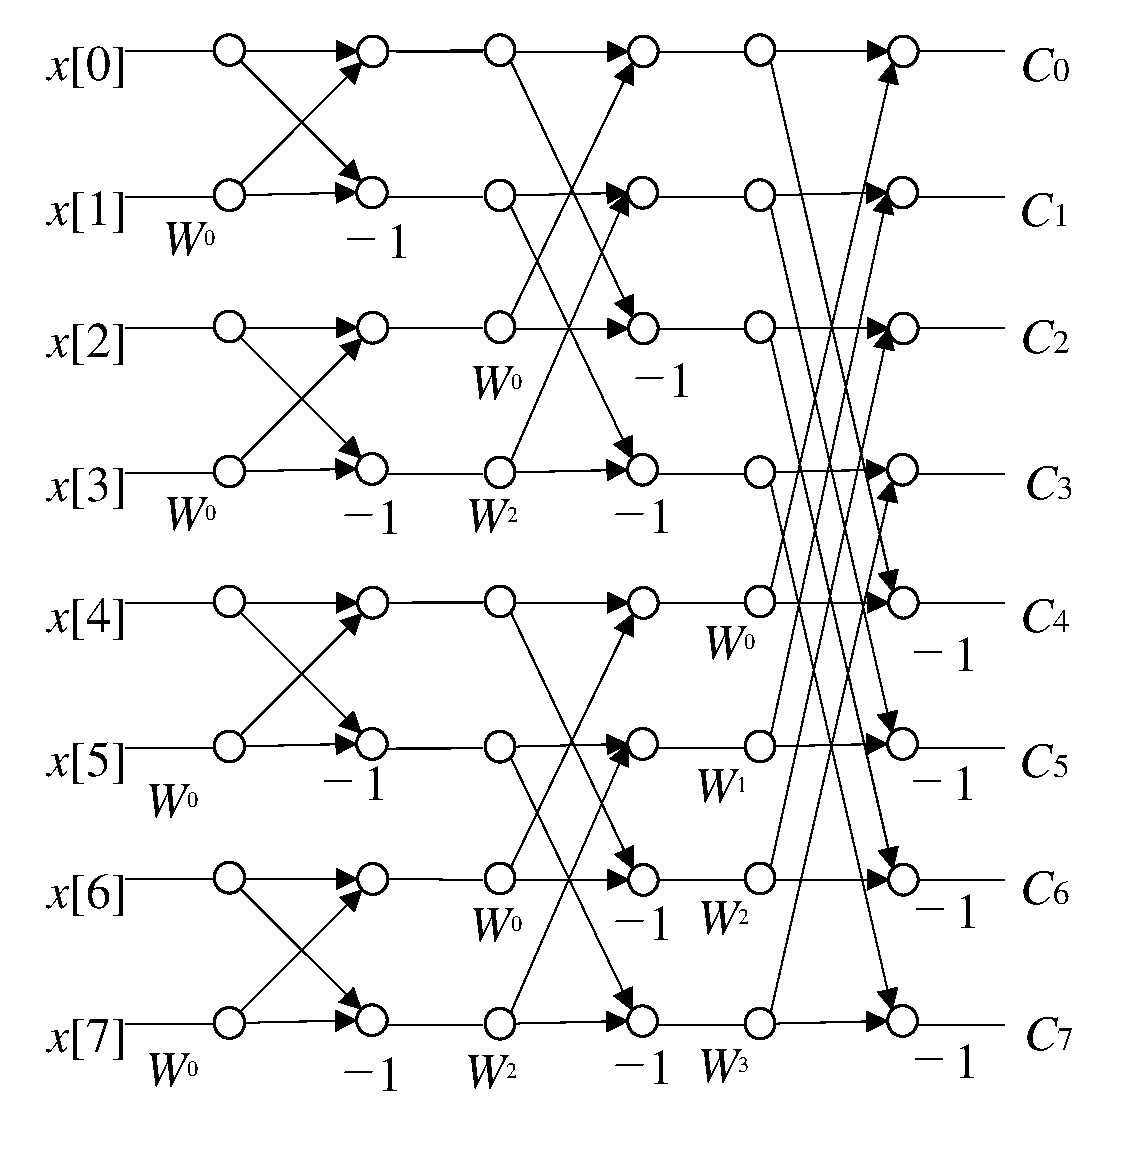
\includegraphics[width=.6\textwidth]{fig/butterfly7.eps}
\end{center}
\caption{8点FFTにおける全体のバタフライ演算}
\label{fig:butterfly8}
\end{figure}

ここで,$N=2^M$であるとすれば,この信号の流れ図は$M$段で構成される.それぞれの段をステージ$L$と呼ぶこととする.この\index{すてーじ@ステージ}ステージ$L$のバタフライ演算を抽出すると,図\ref{fig:butterfly9}のようになる.



\begin{figure}[H]
\begin{center}
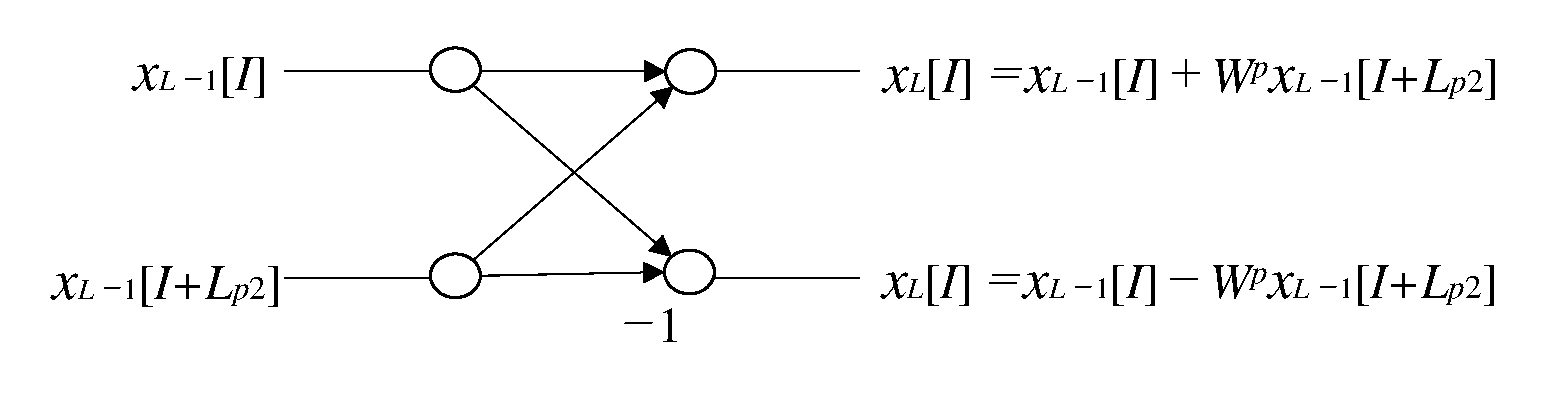
\includegraphics[width=.6\textwidth]{fig/butterfly8.eps}
\end{center}
\caption{ステージ$L$におけるバタフライ演算}
\label{fig:butterfly9}
\end{figure}

ある行番号$I$に対してペアとなる行番号は$I+L_{p2}$となる.ただし,$L_{p2}=L_p/2$,$L_p=2^L$である.
%
それぞれのステージにおいて$N/2$回のバタフライ演算が存在するが,全ステージの出力に掛ける係数$W^p$は各ステージで異なっており,ステージ1では$W^0$だけ,ステージ2では$W^0$と$W^2$,ステージ3では$W^0$~$W^3$となっていることがわかる.
これを表\ref{table:batterfly-p}にまとめる.

\begin{table}[ht]
\caption{バラフライ演算のパラメータ}
\label{table:batterfly-p}
\begin{center}
\begin{tabular}{c|c|c|c|c|c}
\hline
$L$ & 1 & 2 & 3 & $\cdots$ & $N$ \\ \hline
$L_p$ & 2 & 4 & 8 & $\cdots$ & $2^N$ \\ \hline
$L_{p2}$ & 1 & 2 & 4 & $\cdots$ & $2^{N-1}$ \\ \hline
$W^p$ & $W^0$ & $W^0$,$W^1$ & $W^0 \cdots W^3$ & $\cdots$ & $W^0 \cdots W^{L_{p2}}$ \\ \hline
\end{tabular}
\end{center}
\end{table}

ここで$W=e^{-j2\pi /N}$であるから,各ステージの上位におけるバタフライ演算と下位のバタフライ演算との差$D$は,
\begin{equation}
D=-j\frac{2\pi}{L_p}=-j\frac{\pi}{L_{p2}}
\end{equation}
であるので,
\begin{equation}
W^P=e^{DJ} \hspace{1cm} (J=0,1,2, \ldots , L_{p2}-1)
\end{equation}
と書くことができる.そして,それぞれの$W^P$(すなわち角$J$)に対して$I=0$から$L_p$間隔で$N/L_p$回のバタフライ演算を行っている.

このとき,入力データが実数であったとしても,バタフライ演算の過程や最終結果では複素数が存在するため,複素数において実数部と虚数部とに分けて計算をする.
\begin{equation}
x[I]=x_r[I]+j x_i[I]
\end{equation}
\begin{equation}
W^p=e^[DJ]=\cos DJ +j \sin DJ = C+jS
\end{equation}
\begin{equation}
IW = I +L_{p2}
\end{equation}
とおくと,図\ref{fig:butterfly9}の計算は,次式のように書くことができる.

\begin{eqnarray}
x_L{I}&=&x_{L-1}[i]+W^P x_{L-1}[IW] \\
 &=&x_{r(L-1)}[I]+j x_{i(L-1)}[I] \nonumber \\
 & &+ (C+jS)(x_r(L-1)[IW]+j x_{i(L-1)}[IW]) \\
 &=&x_{r(L-1)}[I] + x_{r(L-1)}[IW] C- x_i{(L-1)}[IW] S \nonumber \\
 & &+j( x_{i(L-1)}[I] + x_{r(L-1)}[IW] S+x_{i(L-1)}[IW] C) \\
 &=&x_{r(L-1)}[I] + WR +j( x_{i(L-1)}[I] + WI) 
\end{eqnarray}\vskip.3\baselineskip

\noindent すなわち,
\begin{equation}
x_{rL}[i]=x_{r(L-1)}[I]+WR
\end{equation}
\begin{equation}
x_{iL}[i]=x_{i(L-1)}[I]+WI
\end{equation}
である.ただし,
\begin{equation}
WR=x_{r(L-1)}[IW]C+x_{i(L-1)}[IW]S
\end{equation}
\begin{equation}
WI=x_{r(L-1)}[IW]S+x_{i(L-1)}[IW]C
\end{equation}
\begin{equation}
x_{rL}[IW]=x_{r(L-1)}[I]-WR
\end{equation}
\begin{equation}
x_{iL}[IW]=x_{i(L-1)}[I]-WI
\end{equation}
である.

\section{逆高速フーリエ変換(IFFT)}

離散フーリエ変換
\begin{equation}
X[k]=\frac{1}{N}\sum_{i=0}^{N-1}e^{-j\frac{2\pi}{N}ki} \hspace{5mm} (k=0,1,\ldots , N-1)
\label{eqn:fft01}
\end{equation}
に対する\index{ぎゃくりさんふーりえへんかん@逆離散フーリエ変換}逆離散フーリエ変換は
\begin{equation}
x[i]=\sum_{k=0}^{N-1}e^{j\frac{2\pi}{N}ki} \hspace{5mm} (i=0,1,\ldots , N-1)
\label{eqn:fft02}
\end{equation}
である.
式(\ref{eqn:fft01})と式(\ref{eqn:fft02})を比較すると,偏角の符号と計算結果を$N$で割るかどうかの差異があるということは想像できる.
ここで,FFTと逆高速フーリエ変換(Inverse FFT: \index{IFFT@IFFT}IFFT)との比較を考えることにする.

式(\ref{eqn:fft01})を4点FFTの形式で表すとすれば,次式のようになる.
\begin{equation}
\begin{bmatrix}
X[0] \\
X[1] \\
X[2] \\
X[3]
\end{bmatrix}
=
\begin{bmatrix}
W^0 & W^0 & W^0 & W^0 \\
W^0 & W^1 & W^2 & W^3 \\
W^0 & W^2 & W^4 & W^6 \\
W^0 & W^3 & W^6 & W^9
\end{bmatrix}
\begin{bmatrix}
x[0] \\
x[1] \\
x[2] \\
x[3]
\end{bmatrix}
\label{eqn:fft11}
\end{equation}

式(\ref{eqn:fft02})を同様な形式で表すとすれば,次式のようになる.
\begin{equation}
\begin{bmatrix}
x[0] \\
x[1] \\
x[2] \\
x[3]
\end{bmatrix}
=
\begin{bmatrix}
W^0 & W^0 & W^0 & W^0 \\
W^0 & W^{-1} & W^{-2} & W^{-3} \\
W^0 & W^{-2} & W^{-4} & W^{-6} \\
W^0 & W^{-3} & W^{-6} & W^{-9}
\end{bmatrix}
\begin{bmatrix}
X[0] \\
X[1] \\
X[2] \\
X[3]
\end{bmatrix}
\label{eqn:fft12}
\end{equation}
ここで,$W$の指数が負であることから,対称性と周期性の性質を用いて,
\begin{equation}
\begin{bmatrix}
x[0] \\
x[1] \\
x[2] \\
x[3]
\end{bmatrix}
=
\begin{bmatrix}
W^0 & W^0 & W^0 & W^0 \\
W^0 & W^{3} & W^{6} & W^{9} \\
W^0 & W^{2} & W^{4} & W^{6} \\
W^0 & W^{1} & W^{2} & W^{3}
\end{bmatrix}
\begin{bmatrix}
X[0] \\
X[1] \\
X[2] \\
X[3]
\end{bmatrix}
\label{eqn:fft13}
\end{equation}
ここで,$W$の存在する行列の並びを式(\ref{eqn:fft11})と同様になるように並び換えを行うと,
\begin{equation}
\begin{bmatrix}
x'[0] \\
x'[1] \\
x'[2] \\
x'[3]
\end{bmatrix}
=
\begin{bmatrix}
x[0] \\
x[3] \\
x[2] \\
x[1]
\end{bmatrix}
=
\begin{bmatrix}
W^0 & W^0 & W^0 & W^0 \\
W^0 & W^{1} & W^{2} & W^{3} \\
W^0 & W^{2} & W^{4} & W^{6} \\
W^0 & W^{3} & W^{6} & W^{9}
\end{bmatrix}
\begin{bmatrix}
X[0] \\
X[1] \\
X[2] \\
X[3]
\end{bmatrix}
\label{eqn:fft14}
\end{equation}
と書き表すことができる.このことから,IFFTを行う際は,
\begin{enumerate}
\item $X[k]$のDFTをFFTアルゴリズムにより計算する.
\item 計算における利得$1/N$を修正する.
\item 結果を並び換える.
\end{enumerate}
の3点を注意すれば,先述のFFTアルゴリスムを用いた計算ができるといえる.

\section*{演習問題}

\subsection*{問題\ref{chapter:fft}.1}

図\ref{fig:butterfly8},図\ref{fig:butterfly9}を参考に16点FFTのバタフライ演算を図示せよ.




